\documentclass[a4paper,12pt]{article}

% Font
\usepackage[T1]{fontenc}
\usepackage{gentium}

% Math packages
\usepackage{amsmath}
\usepackage{amsfonts}
\usepackage{amssymb}
\usepackage{amsthm}
\usepackage{bm}

% Define symbol shortcuts
\newcommand{\cc}{\mathcal{C}}
\newcommand{\dd}{\mathcal{D}}
\newcommand{\hh}{\mathcal{H}}
\newcommand{\xx}{{\bm x}}
\newcommand{\yy}{{\bm y}}

% Math environment
\newtheorem*{thm}{Theorem}

% Better list management:
% - vertical spacing in lists
% - items in lists start with dash not bullet point.
\usepackage{enumitem}
\setlist{label=\textemdash,
  itemsep=0pt, topsep=3pt, partopsep=0pt}

% Include graphics
\usepackage{graphicx}
\usepackage{subcaption}

% Page format 
\usepackage[top=2cm,left=2cm,right=2cm,bottom=2cm]{geometry}

\begin{document}
%%% HEADER
\raisebox{0.6in}[0in]{\makebox[\textwidth][r]{\it Unproofed version }}
\vspace{-0.7in}

\begin{center}
\bf\large MA2823: Foundations of Machine Learning \\
Chapter 6: Regularized Linear Regression
\end{center}

\noindent
Lecturer: Chlo\'e-Agathe Azencott   
\hfill
Scribe: Adrien Galamez \\
\null \hfill Paul Magon de la Villehuchet


\noindent
\rule{\textwidth}{1pt}

\medskip

In this chapter we will see:
\begin{itemize}
\item what is regularization;
\item how to use regularization as a means to control model complexity;
\item several forms of regularizing linear regression models.
\end{itemize}

\section{Regression setting}
\subsection{Large $p$, small $n$}
This section is a reminder of the context in which we work. We consider a dataset that has $p$ features and $n$ samples. Thus, we're working with a data matrix $X$ that have $n$ rows and $p$ columns. The outcome vector $y$ describes the quantity we want to predict. The goal of linear regression model is to approximate $y$ as a linear combination of $X$.
\begin{figure}[!h]
\centerline{
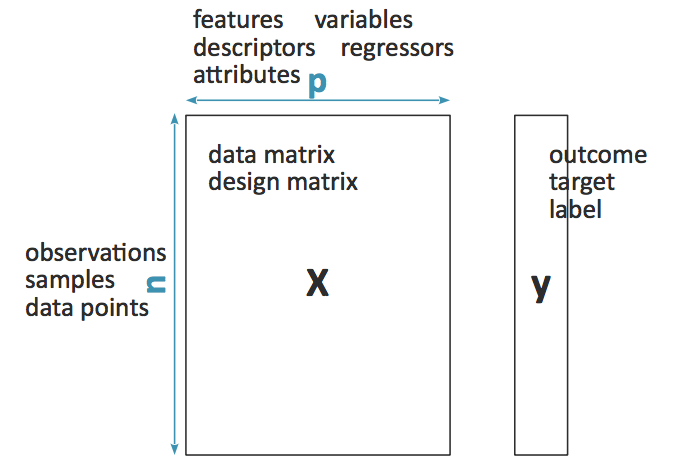
\includegraphics[scale = 0.3]{figures/RegressionSettings.png}}
\caption{Figure illustrating the dimensions of the data matrix and the outcome vector.}
\label{DataMatrix}
\end{figure}

On the Figure \ref{DataMatrix}, we can see that the data matrix is taller than it is wide ($p < n$). This is a  common shape. But, conversed settings can also appear. 

This configuration is called large $p$, small $n$. The data matrix is wider than it is tall. This is the kind of settings we have in genetics and neuroimaging: we have many more descriptors than we have data points. For instance, in genetics, a data set can gather informations for thousands of genes as this information is easy to access. Yet, as each row holds data gathered on a patient, we have at best hundreds of patients. Thus, we have a wide but not tall data matrix. In neuroimaging, brain images are big objets, typically thousands pixels or voxels (3D images). Yet, as brainscans are costly to obtain, we repeat the process on thousands of patient only. Thus, we have more features than observations. In this configuration, regularization is usefull.

\subsection{Linear regression}
\subsubsection{Pro and cons of least-squares fit}
Linear regression is aimed at approximating $y$ as a linear combination of $X$. In the previous chapter, we said that, if we're doing a least-squares fit (which is equivalent to Maximum Likelihood estimation under the assumption of Gaussian noise), we obtain this solution
\begin{equation}
\hat{\beta} = \arg\min_{\beta} (y-X\beta)^{T} (y-X\beta) = (X^T X)^{-1} X^T y.
\label{LR}
\end{equation}
This solution is uniquely defined when $X^T X$ is invertible, hence when $X$ has a full column rank. As $X$ is an $n \times p$ matrix, if $p$ is larger than $n$ (as in the large $p$, small $n$ configuration), $X$ can not be inverted.

This fit has several advantages.
\begin{itemize}
\item The predicted vector $\hat{\beta}$ is unbiased ($\mathbb{E}[\hat{\beta}]= \beta$).
\item If we're restricting to unbiased estimators, minimum mean squared error implies minimum variance.
\item This fit gives an explicit solution (Equation \ref{LR}).
\item If $n \gg p$, the computational time is linear in the number of samples. Indeed, the computational time is $O(\underbrace{np^2}_{\text{compute } X^T X}+\underbrace{p^3}_{\text{invert } X^T X})$. 
\end{itemize}

Yet, this fit has also some drawbacks.
\begin{itemize}
\item Correlated variable leads to high variance of the estimator.
\item Prediction error increases linearly as a function of $p$.
\item The solution is hard to interpret when $p$ is large as shown in the section \ref{LargeP}.
\end{itemize}

\subsubsection{When $p$ in larger than $n$}
\label{LargeP}
When $X^T X$ is not invertible, we still have ways to find $\hat{\beta}$. In this case, we can use the pseudo-inverse of $X$. We can also use numerical methods to solve a linear system of $p$ equations such as gradient descent (aimed at minimizing a convexe function), Gaussian elimination or LU decomposition.
On the Figure \ref{LRPseudoInverse}, we can compare the predicted coefficient (thanks to a linear regression using pseudo-inverse) and the true coefficient when $p = 1000$ and $n = 10$. So, we're in the case of the large $p$, small $n$ configuration. In fact, the outcome vector $y$ was created by a linear combination of the data-matrix $X$ using the weights shown on the left hand graph. 

The objectif was to retrieve those weights using a linear regression on the vectors $X$ and $y$. $10$ causal features were highlighted in orange on both graphs. A good approximation would be to use only those $10$ causal features. Nevertheless, as the right hand graph shows, the linear regression gives coefficients that have approximately the same weight. The causal features are lost entirely in the noise created by the others coefficients. Information has been lost. Regularization is a way of addressing this issue.

\begin{figure}[!h]
\centerline{
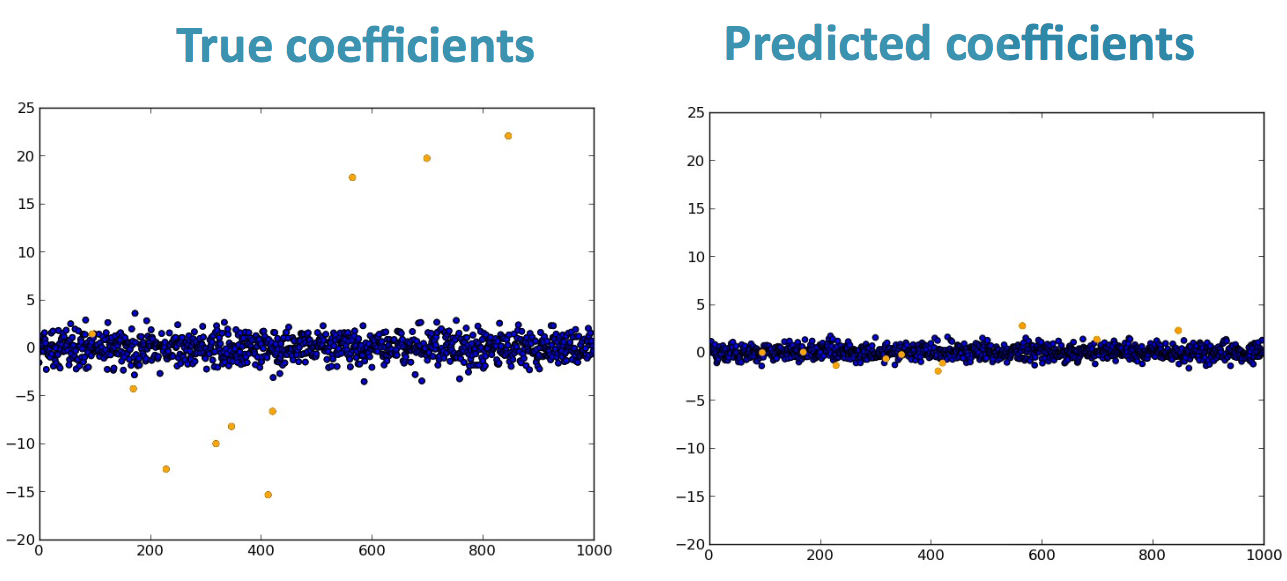
\includegraphics[scale = 0.3]{Figures/linear_regression_pseudoinverse.png}}
\caption{Example of weights obtained from linear regression when $X$ is not invertible, thus using the pseudo-inverse. On the left, the graph is showing the true coefficients of the vector $\beta$. On the right, the graph presents the predicted coefficients of the vector $\hat{\beta}$ obtained from linear regression.}
\label{LRPseudoInverse}
\end{figure}

\section{Regularization}
The Figure \ref{LRPseudoInverse} showed that the linear regression used all the features available to predict the outcome vector $y$. Yet, all the weights are very small. Thus, the solution is hard to interpret. Usually, we prefer having a small subset of features with strong weights. This is one of the advantages of regularization. Moreover, the more we have variables in our model, the more complex our model is. And, the more complex our model is, the more chances we have to overfit our data. Thus, we want to find a way to simplify our model.

 So, instead of minimizing only the sum of squared error, the idea of regularization is to minimize
 \[ \text{Sum of squared error} + \lambda \text{ prenalty on model complexity}.\]
Thus, when using regularization, the estimator is biased (if $\lambda \not = 0$). Yet, because the model will be less complex, we'll have a smaller variance. We're willing to accept a biased estimator in exchange for smaller variance. So, there's a tradeoff to make between bias and variance. $\lambda$ can be set by cross-validation. \label{CVlambda}

This method is also called \emph{shrinkage} in the context of linear regression. Indeed, this is going to shrink the weights of the model. Thus, the final model is simpler.

The following sections are presenting examples of regularization technique.

\subsection{Ridge regression}
\subsubsection{Ridge estimator}
Instead of minimizing our sum of squared error, ridge regression is aimed at minimizing $||y - X\beta||_2^2 + \lambda ||\beta||_2^2$. Thus, the ridge estimator is given by
\[ \hat{\beta}_\text{ridge} = \arg \min_\beta ||y - X\beta||_2^2 + \lambda ||\beta||_2^2. \]

\begin{thm} The ridge regression estimator is given by
\[ \hat{\beta}_\text{ridge} = (X^T X+ \lambda I)^{-1} X^T y. \]
\end{thm}

\begin{proof}
We consider the function $f$ defined by
\[ f(\beta) = ||y - X\beta||_2^2 + \lambda ||\beta||_2^2.\]
In order to minimize this function, we take its gradient.
\[ \nabla_{\beta}f(\beta) = -2X^T (y-X\beta) + 2\lambda \beta.\]
Then, $\beta_\text{ridge}$ is defined as $\nabla_{\beta}f(\beta_{\text{ridge}}) = 0$. Thus,
\[ (X^TX+\lambda I)\beta_\text{ridge} = X^T y.\]
If $\lambda > 0$, $(X^T X + \lambda I)$ is invertible, then
\[ \hat{\beta}_\text{ridge} = (X^T X+ \lambda I)^{-1} X^T y. \]
\end{proof}

\subsubsection{Solution path}
\label{SectionSolutionPathRR}
We've said in section \ref{CVlambda} that we can find the optimal value of $\lambda$ by cross-validation. We can compute solution paths (Figure \ref{SolutionPathRR}) that is a plot showing how the feature coefficient evolves when we decrease the value of $\lambda$. Indeed, when $\lambda = 0$, there's no regularization anymore. And, if $\lambda \gg 1$, we only want to minimize the model complexity. So, all coefficient are then equal to $0$. Then, on the Figure \ref{SolutionPathRR}, on the left hand, we start with the model in which all coefficients are equal to zero and we end, on the right hand, with the linear regression without any regularization model.

The vertical red line shows the value of $\lambda$ that was obtained by cross-validation. The goal is to choose the value of $\lambda$ that gives the best generalization on another set of data.
\begin{figure}[!h]
\centerline{
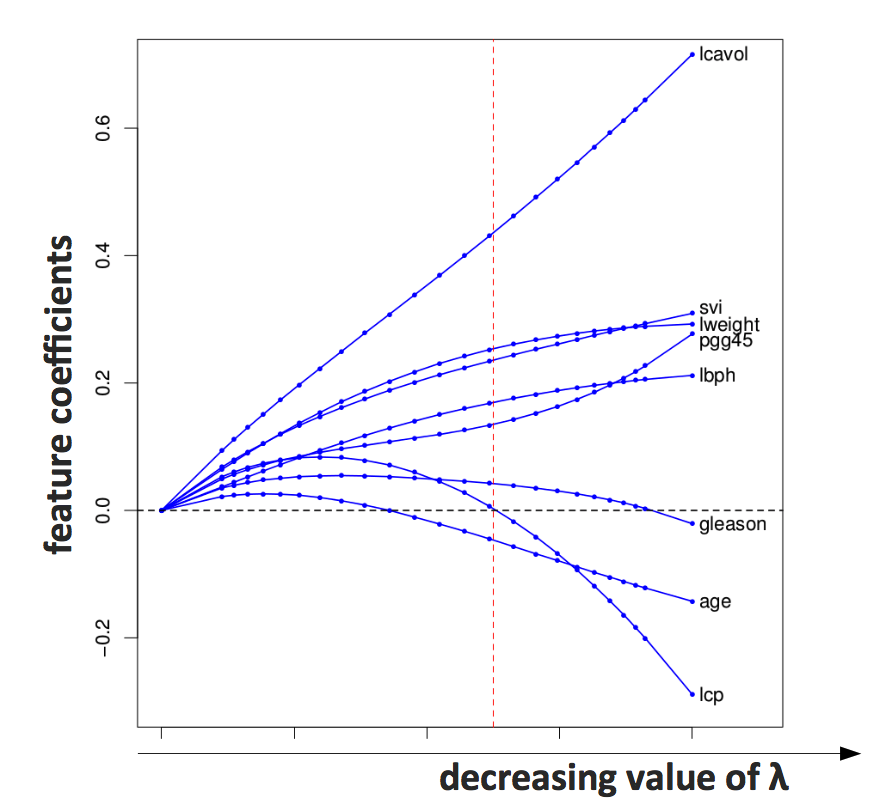
\includegraphics[width = 0.7\textwidth]{figures/solution_path_ridge_regression.png}}
\caption{Ridge regression solution path}
\label{SolutionPathRR}
\end{figure}

\subsubsection{Standardization}
The goal of this section is to describe what will happen to our model if we multiply our features by a constant.
\begin{enumerate}
\item \textbf{Standard linear regression}~: Without any regularization, we multiply, in the data matrix $X$, the column $j$ by a real $c \not = 0$. So, 
\[\forall i \in [|0;n-1|], x_{ij} \to c x_{ij}.\]
Then, the corresponding weight $\beta_j$ is going to be divided by $c$.
\[ \beta_j \to \frac{1}{c} \beta_j.\]
Thus, the weight is different but the solution is similar.
\item \textbf{Ridge regression}~: When we multiply, in the data matrix $X$, the column $j$ by a real $c \not = 0$, we can't know what will happen because of the penalization term $\lambda \beta_j^2$. So, it's important to use standardized feature \emph{before} regularizing linear regression.
\end{enumerate}
\subsubsection{Advantages and drawbacks}
Finally,
\begin{enumerate}
\item \textbf{Advantages}~: Ridge regression has several advantages
\begin{itemize}
\item Correlated variables get similar weights.
\item Identical variables get identical weights.
\item An analytical solution is provided
\end{itemize}
\item \textbf{Drawbacks}~: And it also have drawbacks
\begin{itemize}
\item Ridge regression shrinks coefficients but does \emph{not} result in a sparse model. A model is sparse when many coefficient get a weight of $0$. Then, when a model is sparse, many coefficient can be eliminated from the model.
\end{itemize} 
\end{enumerate}

\subsection{Lasso regression}
\subsubsection{Lasso estimator}
Instead of using the $L^2$ penalty, like the Ridge estimator, the Lasso estimator is based on a $L^1$ penalty. Hence we have to minimize : $||y - X\beta||_2^2 + \lambda ||\beta||_1$.
\begin{equation}
\hat{\beta}_\text{lasso} = \arg \min_\beta ||y - X\beta||_2^2 + \lambda ||\beta||_1.
\label{DefLagrange}
\end{equation}

Unlike the Ridge estimator, there is no explicit solution. We can however, transform this problem into a quadratic problem.

\begin{thm} There is a bijection between $\lambda$ and $t$ such as ${\beta}_\text{lasso}$ is solution of the quadratic problem : 
\begin{equation}
\hat{\beta}_\text{lasso} = \arg \min_\beta ||y - X\beta||_2^2 \quad s.t \quad ||\beta||_1\leq t.
\label{DefQuadratic}
\end{equation}
\end{thm}

\begin{proof}
We consider the functions $f$ and $g$ defined by
\[ f(\beta) = ||y - X\beta||_2^2.\]
\[ g(\beta) = ||\beta||_1 - t.\]
From (\ref{DefQuadratic}) to (\ref{DefLagrange}). Let $H$ be the feasible region, i.e, $\{ \beta$ $, g(\beta) \leq 0\}$
\[ \hat{\beta}_\text{0} = \arg \min_{\beta \in H} ||y - X\beta||_2^2 \quad.\]
Two cases are possible:\\
\begin{itemize}
\item Case 1 : the unconstrained minimum lies in the feasible region. Problem is solved.
\item Case 2 : the unconstrained minimum does not lie in the feasible region. \\
In this case, the solution is the intersection of the iso-contours of $f$ with the boundary of $H$, as shown in the next figure.
\end{itemize}
~\\
\begin{figure}[!h]
\centerline{
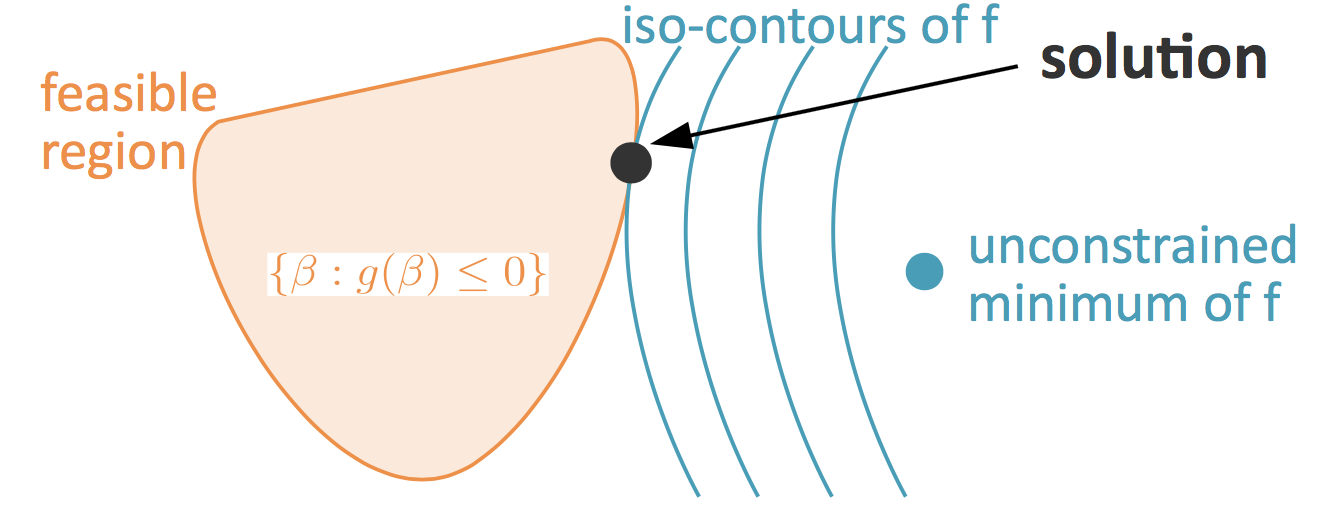
\includegraphics[width = 0.7\textwidth]{figures/sol_lasso.png}}
\caption{Solution of Lasso-estimator}
\label{SolutionLasso}
\end{figure}
~\\
Furthermore, we know that the gradient of $g(\beta)$ is orthogonal to the boundary of $H$.
The gradient of $f(\beta)$ is also orthogonal to the iso-contours of $f$.\\
Hence, at $\beta_{0}$, the gradient of $f$ and $g$ are parallel.\\
We also know that $\nabla_{\beta}g(\beta)$ points towards the unconstrained minimum of $f$ while $\nabla_{\beta}f(\beta)$ points in the opposite direction.\\
~\\
\begin{figure}[!h]
\centerline{
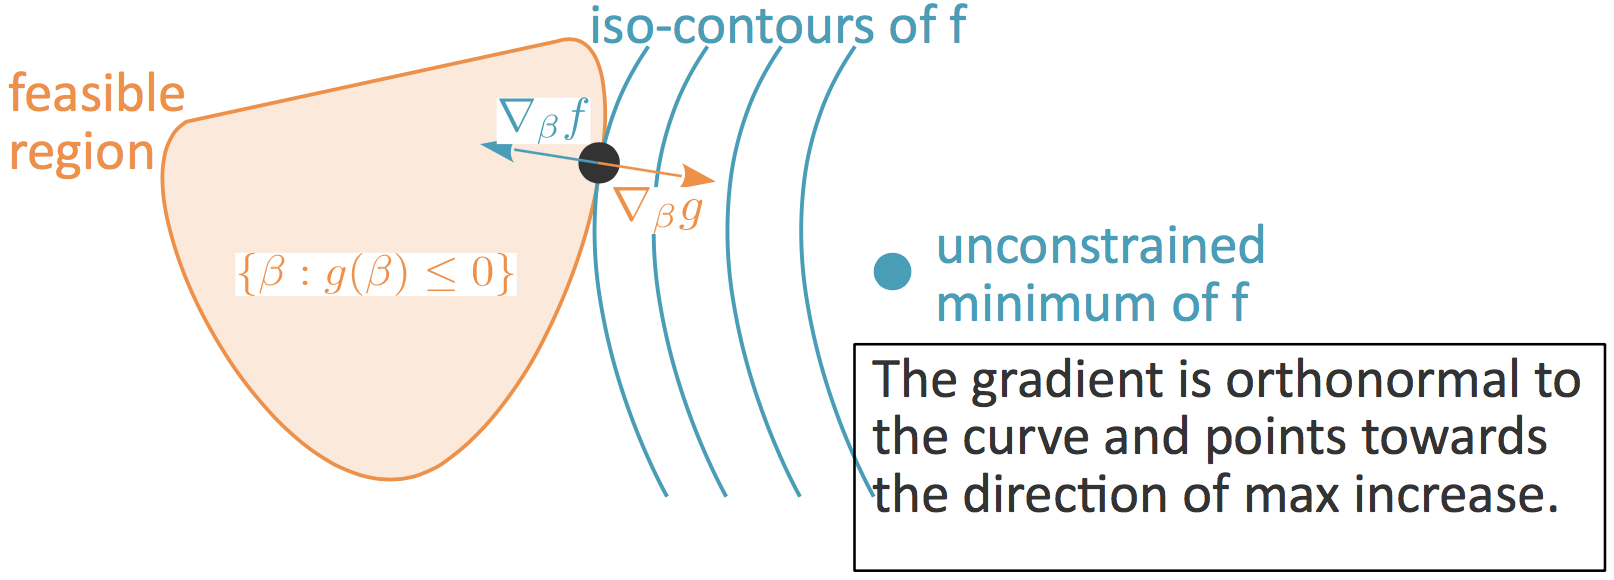
\includegraphics[width = 0.7\textwidth]{figures/sol_lasso2.png}}
\caption{Gradients of $f$ and $g$ and solution of Lasso-estimator}
\label{SolutionLasso2}
\end{figure}
~\\
We can conclude from previous results that $\nabla_{\beta}f(\beta) = -\lambda \nabla_{\beta}g(\beta)$.\\
The Lagrangian of the Lasso-problem : $L(\beta) = f(\beta) + \lambda g(\beta)$ is minimized at $\beta_{0}$. \\

From (\ref{DefLagrange}) to (\ref{DefQuadratic}). Let us fix $\lambda$ and define $\beta_*  = \arg \min_\beta f(\beta) + \lambda ||\beta||_1^2$. Let us define $t = ||\beta_*||_1^2.$\\ 
Then, for any $\beta, f(\beta_*)+ \lambda ||\beta_*||_1^2 \leq f(\beta)+\lambda||\beta||_1^2$. Hence $f(\beta_*)\leq f(\beta)+\lambda(||\beta||_1^2 - t).$\\
Under the constraint that $||\beta||_1^2 \leq t, \lambda(||\beta||_1^2 - t) \leq 0$. Hence $f(\beta_*) \leq f(\beta)$, i.e. $\beta_* = \beta_{lasso}$\\

Thus, the two problems are equivalent.
\end{proof}
\subsubsection{Solution path}
As we did before in Section \ref{SectionSolutionPathRR} for the Ridge Regression estimator, we can also compute solution paths for the Lasso estimator (Figure \ref{SolutionPathLasso}). On the left hand of the graph, we start with high values of $\lambda$ that give very simple models. We move towards lower values of $\lambda$ that gives more complex models. Yet, there's one difference with the ridge regression solution path. In fact, we see here that our features ``enter the model one by one'': their weight is equal to $0$ for all values of $\lambda$ lower to a certain $\lambda_0$. For instance, here, when the model complexity increases, features ``enter'' the model in this order: \texttt{lcavol}, \texttt{lweight}, \texttt{svi}, \ldots, \texttt{gleason}. Thus, at every stage, we have a \emph{sparse model}. For example, on the vertical red line, we have a model with only $5$ parameters that are not null (\texttt{lcavol}, \texttt{svi}, \texttt{lweight}, \texttt{pgg45}, \texttt{lbph}).

\subsubsection{Forward stepwise regression}
We just saw that, in the lasso regularization, the features are ``entering'' the model one by one. Then, we can also get the lasso solution by using forward stepwise regression: the model is built sequentially by adding one variable at a time. Then, this a greedy method.
\begin{itemize}
\item We start with the intercept only.
\item At each step, the variable that most improves the fit is added. All variables are tested and the one that gives the better fit is kept.
\item We stop when $||\beta ||_1 \leq t$.
\end{itemize}

\subsubsection{Least Angle Regression}
The computation of the lasso solution is a quadratic problem, and can be tackled by standard algorithms. But, the least angle regression algorithm is a better approach. In the previous section, when a variable and its weight was added in the model, and this weight was never updated. The least angle regression procedure follow the same general scheme, but doesn't add a feature fully into the model. Here, at each step, ``only as much of a variable as needed'' is added. In fact, the coefficient of that feature is increased only until that feature is no longer the one most correlated with the residual $r$. This algorithms can be described as follow
\begin{enumerate}
\item Standardize the features to have mean zero and unit norm. Start with the residual $r = y - \bar{y}$ and $\beta_1, \ldots, \beta_p = 0$. The residual is ``what is left to explain from our model''. The perfect model would have a residual that is equal to $0$.
\item Find the one feature that explains $r$ the most. In other words, find the feature $x_j$ most correlated with $r$.
\item Update the weight $\beta_j$ until $x_j$ is no longer the one most correlated with $r$: move $\beta_j$ from $0$ towards in the direction of the sign of its correlation with $y$. In fact, move $\beta_j$ from $0$ towards its least-squares coefficient $\langle x_j, r \rangle$ until some other competitor $x_k$ has as much correlation with the current residual as does $x_j$. So
\[ \beta_j + \alpha \frac{1}{\sum_{i=1}^n (x_j^i)^2} \sum_{i=1}^n x_j^i r^i \to \beta_j,\]
\[ (y - \bar{y}) - \beta_j x_j \to r,\]
where $\alpha$ is called the step size.
\item Move $\beta_j$ and $\beta_k$ in the direction defined by their joint least squares coefficient of the current residual on $\langle x_j, x_k \rangle$ until some other competitor $x_l$ has a much correlation with the current residual $r = (y-\bar{y} - \beta_j x_j - \beta_k x_k)$.
\item If a non-zero coefficient hits zero, drop its variable from the active set of variables and recompute the current joint least squares direction.
\item Continue in this way until all $p$ predictors have been entered.
\end{enumerate}

\begin{figure}[!h]
\centerline{
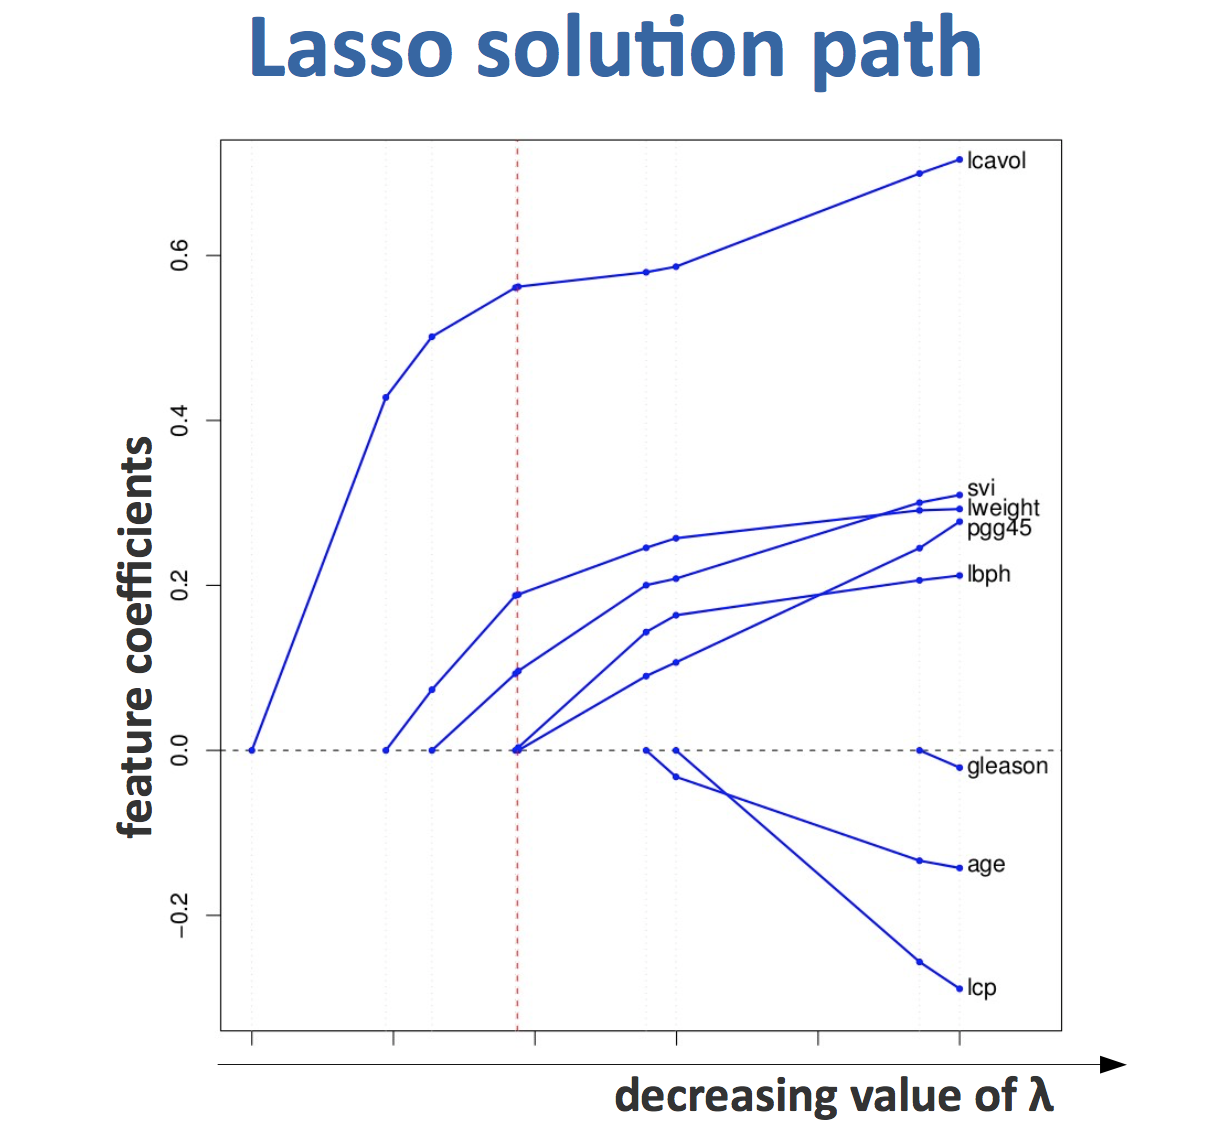
\includegraphics[width = 0.7\textwidth]{figures/solution_path_lasso.png}}
\caption{Ridge regression solution path}
\label{SolutionPathLasso}
\end{figure}

\subsection{Elastic Net}
\subsubsection{Elastic Net estimator}
The Elastic Net estimator is a convex combination of Lasso and Ridge. It is defined by :
\[ \hat{\beta}_\text{enet} = \arg \min_\beta ||y - X\beta||_2^2 + \lambda(\alpha||\beta||_2^2 + (1 - \alpha)||\beta||_1) \]
The main advantage is to combine both :
\begin{itemize}
\item It selects variables like the Lasso-estimator. 
\item It shrinks together correlated and identical variables like the Ridge-estimator
\end{itemize}
Of course, this cames with the cost of having two parameters ($\lambda$, $\alpha$) to set instead of one.

\subsubsection{Comparison of Elastic Net-estimator and Lasso-estimator}
The Figure \ref{Lassoenet} represents results of both Lasso-estimator and Elastic Net-estimator on Leukemia data. We can see that Elastic Net results in more non-zero coefficients than Lasso, but with smaller amplitudes.

\begin{figure}[!h]
\centerline{
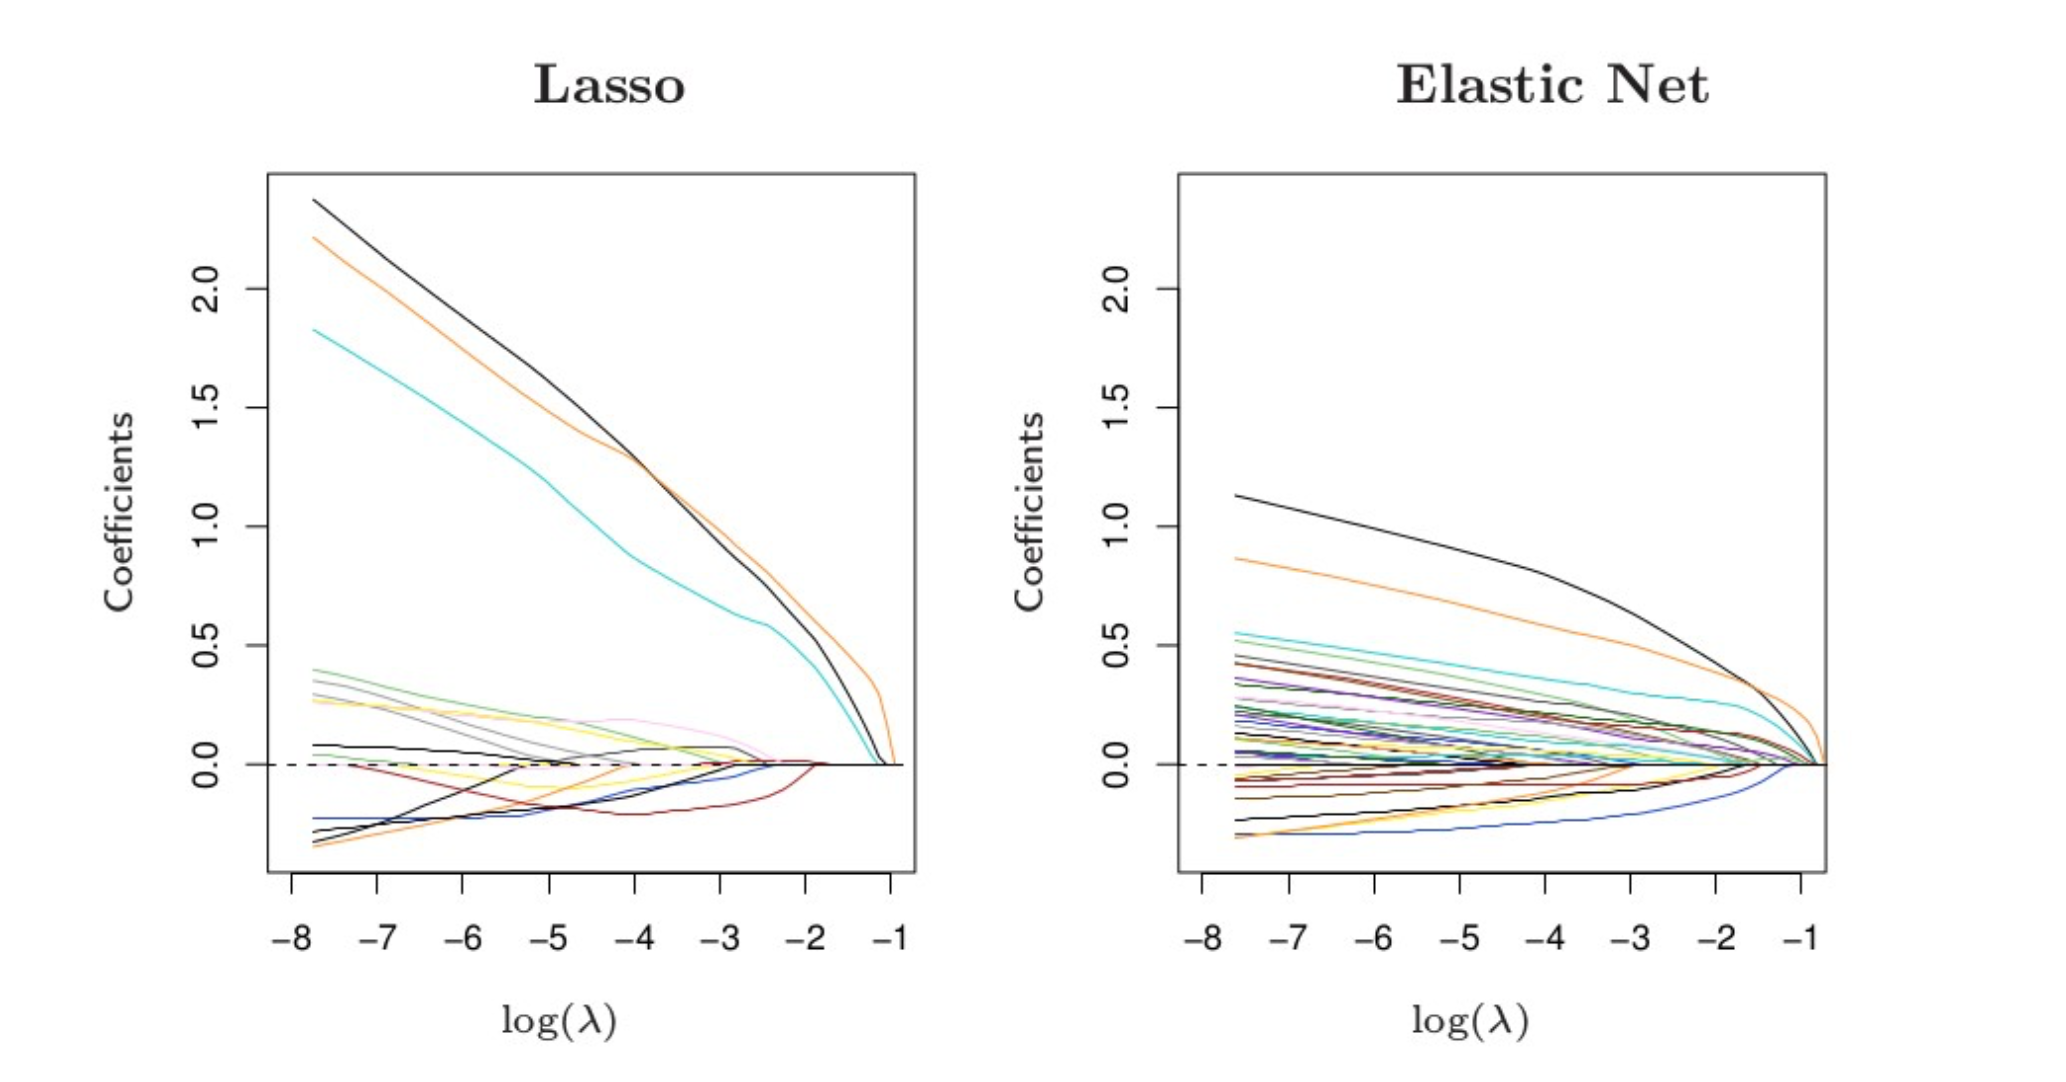
\includegraphics[width = 0.9\textwidth]{figures/lassoenet.png}}
\caption{Comparison of weights on Lasso-estimator and Elastic Net estimator}
\label{Lassoenet}
\end{figure}

\subsection{$L^q$ regression}
\subsubsection{$L^q$ estimator}
The $L^q$ estimator is a generalization of the Ridge and Lasso estimator : the penalty is based on the $L^q$ norm of $\beta$.
\[||\beta||_q^q = \sum_{i = 1}^{n}{\beta_{i}^q}\]
The $L^q$ estimator is then defined by :
\[ \hat{\beta}_\text{$L^q$} = \arg \min_\beta ||y - X\beta||_2^2 + \lambda ||\beta||_q^q. \]
We have the same theorem to transform this problem into a quadratic problem with constraints.\\

\begin{thm} There is a bijection between $\lambda$ and $t$ such that ${\beta}_\text{$L^q$}$ is solution of the quadratic problem : 
\[ \hat{\beta}_\text{$L^q$} = \arg \min_\beta ||y - X\beta||_2^2 \quad s.t \quad ||\beta||_q^q\leq t. \]
\end{thm}

\begin{proof}
The proof follow the same steps than the previous one.
\end{proof}

The Figure \ref{Bound2} represents the feasible sets for different values of $q$.
\begin{figure}[!h]
\centerline{
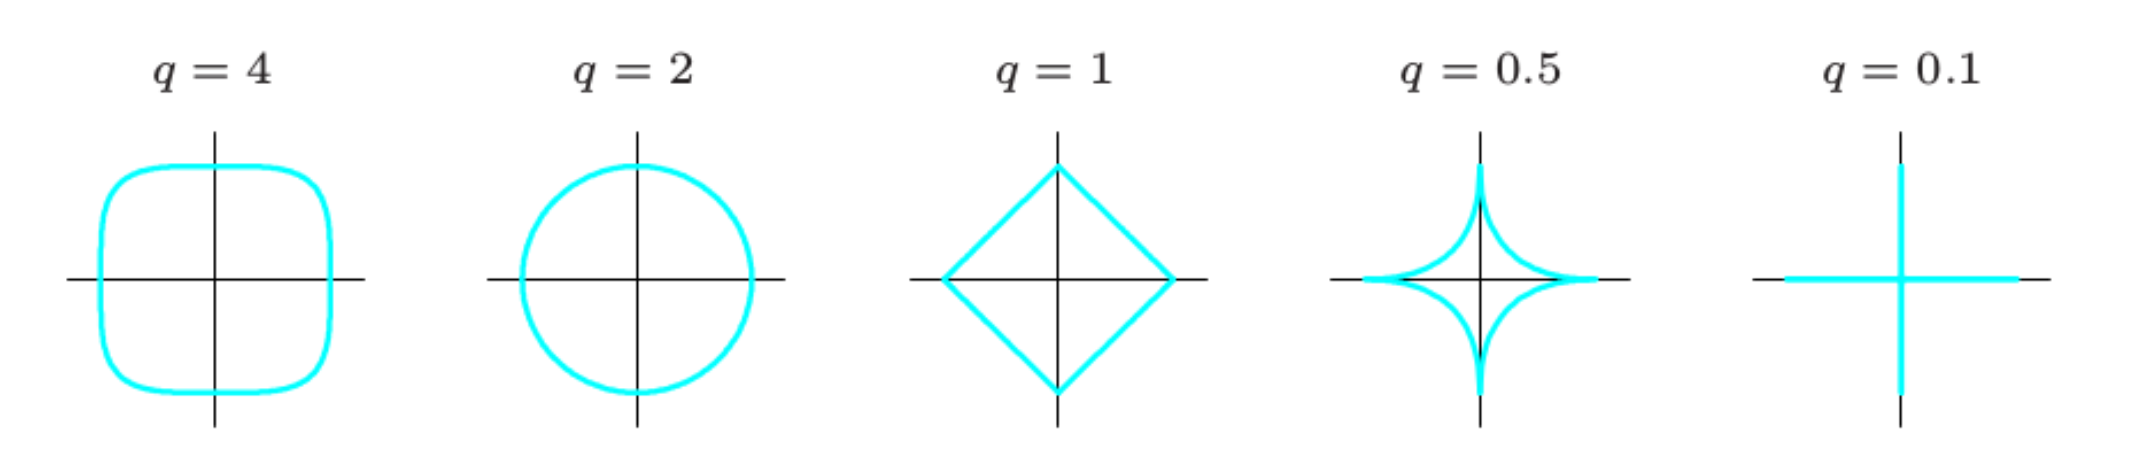
\includegraphics[width = 0.7\textwidth]{figures/bound.png}}
\caption{Boundaries of the feasible set with different values of q}
\label{Bound2}
\end{figure}

\subsubsection{Comparison between Lasso and Ridge}
Because the feasible depends on the value of $q$, the Ridge $(q = 2)$ and Lasso $(q = 1)$ estimator will be different. The feasible set will be a square in one case and a circle in the other. This helps understand why the $L^1$ norm gives sparse models. Indeed, the $L^1$ ball has corners. This means that when we're moving from the unconstrained minimum towards the ball, we're more likely to ``hit'' a corner of the ball. And, on a corner of the ball, only one feature has a weight non equal to zero.

\begin{figure}[!h]
\centerline{
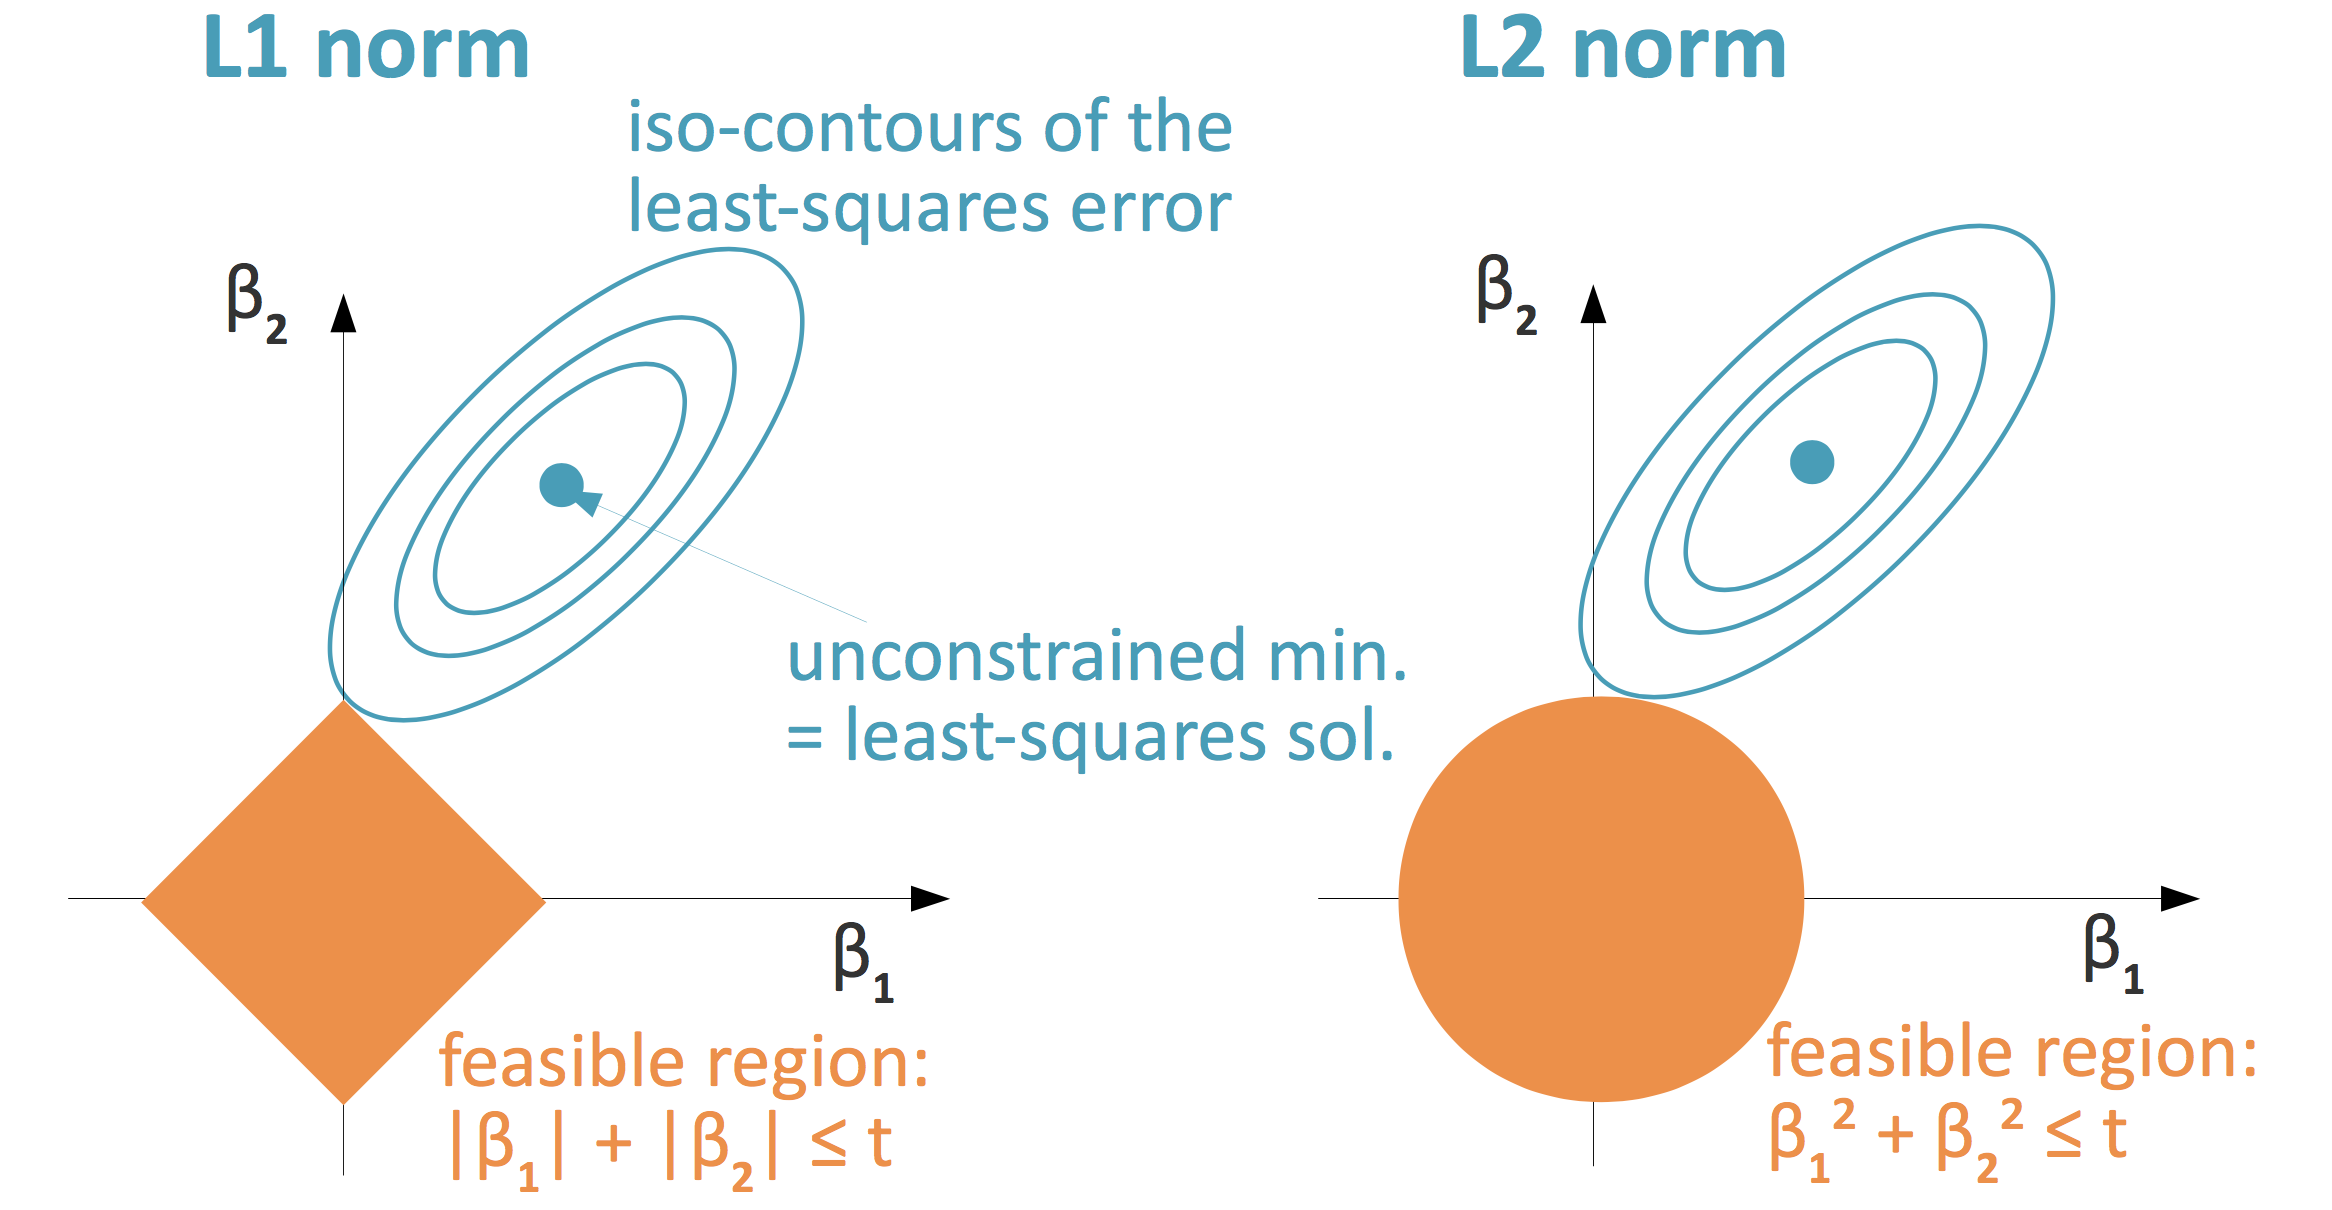
\includegraphics[width = 0.7\textwidth]{figures/comparison.png}}
\caption{Comparison of the Lasso-estimator and the Ridge-estimator}
\label{Comparison}
\end{figure}

\subsection{Structured Regularization}
\subsubsection{Group Lasso}
The \emph{group Lasso} is a variant of Lasso. All $p$ variables are partitioned in $K$ predefined groups of variables that are known to work together and expected to work together and thus be all active or inactive together. For instance, genes belonging to the same biological pathway can form a group.

Let $X_k$ be the features belonging to group $k$. Let $p_k$ be the size of group $k$. We have : $\sum_{k = 1}^K{p_k} = p$. We can define the Group Lasso-estimator:
\[ \hat{\beta}_\text{grlasso} = \arg \min_\beta ||y - \sum_{k = 1}^K{X_k\beta_k}||_2^2 + \lambda \sum_{k = 1}^K{\sqrt{p_k}||\beta_k||_2}\]

\subsubsection{Other structured penalties}
Other regularizations exist :
\begin{itemize}
\item Overlapping groups
\item Graphs
\item Trees
\item Multiple related Tasks
\end{itemize}

\section{Conclusion}
We've replaced the minimization of the sum of squared errors (that gave us the solution of the linear regression problem) by minimizing the sum of squared errors \emph{plus} a regularizer that penalizes the model complexity. We've seen 3 major forms of regularizers:
\begin{itemize}
\item Ridge regression ($L^2$ norm)
	\begin{itemize}
	\item gives similar weights to similar variables,
	\item doesn't really give sparse solution,
	\item but has the advantage of having an explicit solution.
	\end{itemize}
\item Lasso regression ($L^1$ norm)
	\begin{itemize}
	\item randomly picks one of several correlated variables,
	\item gives sparse solution,
	\item can be implemented by the Least Angle Regression algorithm.
	\end{itemize}
\item Elastic net (combining $L^1$ and $L^2$ norm)
	\begin{itemize}
	\item selects variables like the lasso,
	\item shrinks together the coefficients of correlated variables.
	\end{itemize}
\end{itemize}

\end{document}